\documentclass[11pt]{article}
\usepackage{amsmath,amsfonts}
\usepackage[numbers,sort&compress]{natbib}
\usepackage{times}
\usepackage[left=2.54cm,top=2.54cm,right=2.54cm,bottom=2.54cm,bindingoffset=0.0cm]{geometry}
\usepackage{setspace}
\usepackage{enumerate}
\usepackage{enumitem}
\usepackage{wrapfig}
\setcounter{secnumdepth}{0}
\usepackage{fullpage}
\usepackage{titlesec}
\titleformat{\section}{\large\bfseries}{\thesection}{1em}{}
\titleformat{\subsection}{\bfseries}{\thesubsection}{1em}{}
\usepackage{parskip} % skip paragraph indentations
\usepackage{lipsum}
\usepackage{hyperref}
\usepackage{graphicx}
\usepackage{amssymb}
\usepackage[x11names]{xcolor}
\usepackage{hyperref}
\usepackage{enumitem}
\usepackage{booktabs}
\usepackage{amsmath}
\usepackage{amssymb}
\usepackage{mathrsfs}
\usepackage{caption} \captionsetup[table]{singlelinecheck=false} %makes table captions left-justified
\usepackage{framed} % to add frames around comments
%\hypersetup{backref,colorlinks=false,
%    urlbordercolor=LightSkyBlue4,          % color of internal links
%    citebordercolor=SpringGreen4,        % color of links to bibliography
%    filebordercolor=magenta,      % color of file links
%    linkbordercolor=Red3, pdfborderstyle={/S/U/W 1.5}}
\newcommand{\Prob}[1]{\Pr{\left( #1 \right)}}
\newcommand{\q}[1]{``#1''} % easier way to get double quotes
\newcommand{\argmin}{\text{argmin}}
\usepackage{authblk} % for title page
\renewcommand\Affilfont{\fontsize{10}{10.8}\itshape}
\renewcommand\familydefault{\sfdefault} 
\usepackage{datetime2}
%\renewcommand{\dateseparator}{-}
\usepackage{atbegshi}% http://ctan.org/pkg/atbegshi -- removes blank page at start of doc
\AtBeginDocument{\AtBeginShipoutNext{\AtBeginShipoutDiscard}}
\setcounter{page}{0}

\lhead{Learning strategies for quality assessment} 

%maybe a broader title? but we don't want to get in to the social learning of tasks/behaviors areas, so we'll have to be careful with the wording...

%\lhead{Large groups and poor memory favor learning about badges}


\begin{document}
\noindent
\title{Learning strategies for quality assessment: the tradeoff between general rules and recognition} 
\author{}
\date{} 
\maketitle

%New target journal: Proc B 
%instructions: http://rspb.royalsocietypublishing.org/author-information
% open access: https://royalsociety.org/journals/authors/open-access/

%%%%%%%%%%%%%%%%%%%%%%%%%%%%%%%%%%%%
\linenumbers

\section*{Lay summary}
Animals that live in groups often need accurate information about their group mates, but there are several ways that this assessment can work. Some animals learn to recognize something about others, and sort individuals into categories or remember particular individuals, but others may learn general rules of thumb that apply to all individuals. We find that recognition learning is always more difficult than rule learning in large groups and when animals have poor memory. In these cases, it is better to learn about general rules of quality, rather than relying on learning about to recognize individuals.

% % TERMS:
% recognition vs rule learning strategies
% individual recognition vs categorical recognition


%%%%%%%%%%%%%%%%%%%%%%%
\section*{Abstract}
%%%%%%%%%%%%%%%%%%%%%%%
Animals in social groups benefit from having accurate information about their group mates. Different species have different methods for gathering this information: some animals recognize members of their groups as individuals, while others coarsely categorize conspecifics based on observable traits. In many animals, a property of interest, for example dominance or health, is correlated with an otherwise unimportant trait, which is then referred to as a badge of status. Much is known about the circumstances that promote the evolution of either individual recognition or a badge of status, but there are few studies that compare the effectiveness of the two systems of learning. In order to study how group size and cognitive abilities influence the effectiveness of both types of learning and to determine the circumstances under which one is preferable, we develop and analyze a simple model of an animal social group, in which animals learn by interacting with each other and by observing these interactions. Regardless of how the animals assess the quality of their group mates, we find that larger group sizes and longer memory windows make it easier to learn more accurately and more quickly. We also find that intermediate perceptive abilities maximize the effectiveness of learning about a badge of status and that observational learning is more beneficial for animals using individual recognition. Finally, we find that learning about a badge of status is less costly than individual recognition when animals live in large groups, have short memories, and have coarse perceptive abilities.



\textbf{Keywords:} badge, cognition, evolution, learning, recognition, signal, social groups

\newpage
%%%%%%%%%%%%%%%%%%%%%%%
\section*{Introduction} 
%%%%%%%%%%%%%%%%%%%%%%%
Animals in social groups benefit from having accurate information about their group mates \citep{Seyfarth:2010bh}. Knowledge of the dominance ~\citep{Waal:1986ys,Cowlishaw:1990vn,Bergman:2003qf,Seyfarth:2005ve,Flack:2006uq,Hobson:2015uq}, resource holding potential~\citep{Rhijn:1980uq,Freeman:1985kl,Dick:1990cr,Lemel:1993ve}, likelihood of investing in parental care~\citep{Qvarnstrom:1997fk,Olsen:2010uq}, or health~\citep{Folstad:1992kx,Loyau:2005nx} of other animals can help an animal decide with whom to fight, mate, or interact. There are several ways animals may learn about their group mates when the quality of individuals varies. First, animals can use recognition, either to recognize specific individuals, or to recognize the discrete quality category in which an individual belongs. In some animals, a quality property of interest, for example dominance or health, is correlated with an otherwise unimportant trait, which is then referred to as a badge of status~\citep{dawkins1978signals,Rohwer:1981vn,Rohwer:1982fk} and can allow animals to make inferences about each others' quality as mates or opponents or allies at the categorical level. Second, animals can use generalizable rules of thumb, where they must learn the rule that links quality and signal in order to infer quality in a continuous pattern.  

%pitch for paper
Much is known about what circumstances might promote the evolution of recognition-based or rule-based learning (e.g. \citep{Whitfield:1987tg,Rohwer:1975fk,Lemel:1993ve,Solberg:1997uq,Tibbetts:2009kx,Remy:2010fk,Sheehan:2014fk}), but there are few studies that compare the two systems directly \citep{sheehan2016evotradeoff}. Our goal in this paper is to compare the relative costs of learned recognition with learned rules for assessing the quality of others. We developed and analyzed an agent-based model of a simple animal social group, in which animals learn about each other through dyadic interactions. We then study how group size and cognitive abilities influence the effectiveness of both types of learning and to determine the circumstances under which one is preferable.  

% summary of previous research on continuous learning (rules)
%In contrast to recognition-based learning, 
Individuals can use more continuous rule-based strategies to learn about each other's quality. Here, rather than learning to recognize individuals, each animal is learning the general underlying rule for the distribution of quality among individuals in their groups. An example of this is a 'rule of thumb' that individuals may follow to make decisions. [TKTK more needed here] 

% to add: size or age-based ranking systems would be a good rule of thumb


% summary of recognition-based learning
Many species use a recognition-based learning system in order to evaluate each other. At the most detailed level, individuals learn about specific others using individual recognition. Here, knowing something about the quality of one particular individual does not allow the animal to infer anything about the quality of other individuals. At a more general level, individuals learn about others by recognizing the category to which that individual belongs. This type of recognition does allow for animals to inference quality beyond particular individuals, and to assign all individuals that fall into a certain category the same level of quality. Depending on the number of categories that individuals can be sorted into, this type of assessment can be relatively detailed (where many categories are perceptible) or provide only basic information about quality (where few categories are available to assign individuals to, so there is a larger range of quality among same-classed individuals). One example of categorical recognition is badges of quality, where a signal can be used by others to make inferences about the quality of the individual. 

%rational for grouping these together
While categorical sorting (e.g. by badges of status) and individual recognition are usually presented as fundamentally different solutions to the same biological problem (e.g. see \citep{sheehan2016evotradeoff}, individual recognition is in some ways just an extreme version of learning about others' categorical quality \citep{Barnard:1979fk}. If an animal has a limited ability to tell the difference between two animals with similar categories, it will classify both individuals into the same category and therefore the same ``quality." As the magnitude of the difference in categories an animal can perceive gets smaller and smaller, eventually it will be able to recognize each of its peers individually. Such a spectrum from coarse-grained to fine-grained perceptive abilities can be seen in some real world examples. Within paper wasps, some species distinguish between other wasps based on the number of black patches on their face, a relatively coarse trait \citep{Tibbetts:2004kx}, whereas in other species, wasps can recognize specific individuals based on their unique facial patterns \citep{Tibbetts:2002ys}. 

Where a species sits on this spectrum depends on their cognitive abilities. The specificity with which animals can distinguish a trait also depends on the the type of variation present in the trait. A bimodally distributed trait can easily be divided into ``small" or ``large" categories, while a normally distributed trait may necessitate further subdivision. Indeed, there are some species of birds whose populations exhibit bimodally distributed badges of status and others whose populations exhibit normally distributed badges \citep{Ripoll:2004vn}.

The correlation between the category or badge and another trait has been the focus of many previous studies, as described above. However, the specificity with which the badge can be perceived has not been as well studied. As we show below, this is a crucial factor in determining how effectively an animal can learn from its group mates' badges. Because the two systems are usually thought of as totally separate, they are usually studied separately \citep{sheehan2016evotradeoff}. In this paper, we explicitly compare the performance of animals using types of learning that fall across this spectrum with a more general rule-based learning system.

% How to learn
Regardless of whether animals pay attention to a quality category or focus on individual identity, they have several potential sources of information. 

Regardless of whether animals utilize a recognition-based or rule-based quality assessment strategy, they can learn about quality through both  directly experienced interactions, and those that they observe as bystanders. For example, when two pigtailed macaques fight, they both gain direct information about the other's ability through experiencing the fight, which they keep track of over time \citep{Flack:2006uq}. animals can also learn through observational learning. By observing the result of interactions between other pairs of animals, one can gain information about their relative abilities or sometimes even their absolute abilities. Observational learning has been observed in many species (e.g. \citep{Gaudet:1984cr,Holekamp:1991nx,Fiorito:1992ve,Marchetti:2000dq,Bugnyar:2002qf,Hopper:2008bh,Hobson:2015uq}). It is a valuable way of gathering information \citep{Holekamp:1991nx,Schaik:2011oq,Seyfarth2015SocialCognition}, especially for animals trying to learn about other members of their social group \citep{Freeman:1985kl,Holekamp:1991nx,Hobson:2015uq}. However, the degree to which it helps an animal learn depends on the information it already has and the advantage of using observational learning may differ depending on what kind of learning an animal engages in.


% LEARNING ABOUT QUALITY
Many factors influence how accurately animals can learn about their group mates. Sheehan and Bergman~\citep{sheehan2016evotradeoff} predicted that group size, the stability of the social group, and the stability of the quality signal over time should all affect how well animals using recognition-based systems can learn about their peers. [TKTK something about rules]

%cognitive constraints on learning
The systems that individuals use to assess each other are likely subject to cognitive constraints. For example, in individual recognition, as groups become larger and larger, it becomes more difficult to effectively and accurately learn about and remember assessments for all of one's group mates \citep{Rohwer:1982fk,Solberg:1997uq}. Learning about relative quality rankings or relationships between individuals quickly becomes combinatorially explosive~\citep{Seyfarth2015SocialCognition}. Even humans are thought to be limited in terms of individual recognition. Previous work has hypothesized that humans can only remember the faces of about 150 people \citep{Dunbar:1993zr,Hill:2003ly}. These cognitive constraints may have been important in early human evolution, especially in the context of cooperation, and may in turn have imposed social constraints, limiting early human group sizes~\citep{Dunbar:1992ys,Dunbar:1993zr}.


In this paper, we focus on the effects of group size and cognitive traits. Our goals are (1) to investigate how group size, memory, and perceptive ability alter the extent to which animals can learn the quality of their group mates, (2) to evaluate how observational learning affects how well can animals can learn, and (3) to determine the conditions under which the evolution of learning based on a badge signal or learning based on individual recognition would be favored. To address these questions, we develop a model, in which quality assessment occurs by one of two methods: (A) a badge system, where animals assess the quality of others by grouping individuals into categories based on the intensity of their badges and (B) an individual recognition system, where animals can assess the quality of specific individuals.  


%%%%%%%%%%%%%%%%%%%%%%%
\section*{Model} 
%%%%%%%%%%%%%%%%%%%%%%%

In this paper, we study a simple model of an animal social group in which animals assess each other and incur costs based on these assessments. Generally, each animal in a social group has an inherent quality value. This can be thought of, for example, as fighting ability, resource holding potential, body size, body condition, or any other property about which it would be beneficial to have accurate information. Animals can acquire information about their peers in several ways. Some animals can recognize their peers, based on visual, olfactory, or auditory traits, and then learn about the quality of each of their peers over the course of time \cite{sheehan2016evotradeoff}. An animal may be limited in its ability to distinguish its peers by its perceptive ability. For example, if it cannot distinguish similar colors from each other, it would think two similarly-colored animals are the same and would therefore confuse their quality values as well. On the other hand, an animal can use a rule-of-thumb to infer the quality values of its peers from a signal that they display. Such a rule can be innate or it can be learned over time, as an animal learns the relationship between a property of interest and another trait. 

Animals use information about their group mates to decide how to interact with them in the future. Therefore, if animals learn about each other inaccurately, they will make inappropriate decisions and incur costs. The time spent interacting with and observing one's group mates could be spent in other ways, and if the interaction is actually a fight, having more interactions than necessary can lead to injury and perhaps even death.  Therefore, the longer it takes to acquire an accurate estimate, the more costs the animals incur. Waiting longer and gathering more information tends to improve the accuracy of an animal's assessment, so there is an inherent tradeoff between accuracy and speed. In different species, accuracy and speed may be more or less important and how they are combined to affect an animal's total fitness is an important consideration in understanding the optimal learning strategy. We now describe the specific details of the model. 

\subsection{Interactions and learning }
We consider a group of animals containing $N$ individuals. (See Table~\ref{tab:vars} for a description of all of the parameters used in the text.) We assign each animal a quality value, $q_i$, and a signal, $s_i$. We consider three ways in which animals assess each other: recognition, an innate rule-of-thumb, and a learned rule-of-thumb. With recognition, the signal is the trait that animals attend to in order to recognize their group mates. With a rule-of-thumb, the animals use either an innate or a learned relationship between the signal and quality to infer the quality of any particular group mate. Specifically, we draw quality values $\{q_1,\dots,q_N\}$ from a normal distribution with mean $0$ and standard deviation $\sigma_\text{q}$. We then generate $N$ signal values $\{s_i\}$ such that 
%$\min_i{s_i}\approx -1$, $\max_i{s_i}\approx 1$, and 
$\max_i\{s_i\}-\min_i\{s_i\}=2$ and the sample correlation between $\{q_i\}$ and $\{s_i\}$ is precisely $\rho$. 
The higher $\rho$ is, the more informative the signal is about the underlying quality of the animals.

With recognition, animals will try to learn about the quality of each of its group mates. However, they are potentially limited by their perceptive abilities. Specifically, an animal can only distinguish between two other animals $j$ and $k$ if $|s_j-s_k|>\delta$, that is, if their signals are sufficiently different. If the animals have fine perceptive abilities, the parameter $\delta$ will be small, and if the animals have coarse perceptive abilities, the parameter $\delta$ will be large. For example, if $\delta$ is be large, an animal can only discriminate among animals with small, medium, and large signals, and the best it can do is to learn about the quality of all animals in each of these three categories. On the other hand, if $\delta=0$, an animal can discriminate every individual in its group and it can learn about the quality of each. Before any interactions take place, each animal in the group divides its peers into categories. It does so by picking another animal, $j$, at random. All animals whose signals are within $\delta/2$ of $s_j$ are put in the same category. Then the focal animal picks an uncategorized animal at random, $k$, forming a second category of all uncategorized animals whose signals are within $\delta/2$ of $s_k$. The process continues until every animal in the group has been assigned a category. The parameter $\delta$ can therefore be thought of as ``category width."  Different animals will categorize the group differently and may perceive different numbers of categories. Figure \ref{cats_ex} shows one example of this process for various values of $\delta$. When $\delta=0$, there are as many ``categories" as there are animals, and as category width increases, the average number of categories animals recognize decreases (Figure \ref{num_cat}). Since we analyze the effects of several parameters, we could not explore every possible value of each parameter. Rather, we choose a representative set of values. In particular, we allow $\delta$ to take on the values $0$, $0.25$, $0.5$, $0.75$, and $1$.

Each animal $i$ has an assessment of each other animal $j$ at each point in time $t$, $a_{ij}(t)$.  At first, the group consists entirely of naive animals: at $t=0$, no animal has an opinion of any other. At each timestep, the animals forget their assessments of animals they have not interacted with recently: if an animal has not updated its opinion of animals in a given category within the last $w$ timesteps, it forgets its opinion of that category, so that $w$ can be described as the animals' ``memory window." Next, two animals, $i$ and $j$, are chosen randomly to interact. Through this interaction, each receive noisy information about the other's quality. Each animal then updates its assessment of the other to be the weighted average of its old estimate and the new information it has received. Specifically, if $i$ already has an opinion of $j$, its new estimate is
\begin{equation*}
a_{ij}(t+1)=(1-r)a_{ij}(t)+r(q_j+\xi),
\end{equation*}
where $r$ is the ``updating rate" describing how much each animal changes its assessment based on the interaction and $\xi$ is drawn from a normal distribution with mean $0$ and standard deviation $\sigma_\xi$. As with $\delta$, we choose a representative set of values of $r$ to explore, specifically, $0.05$, $0.1$, $0.25$, and $0.5$. It simultaneously updates its opinions of all the other animals in the same category as $j$.
If $i$ has not previously interacted with animals in $j$'s category or if $i$ has forgotten about the category, $i$'s new estimate of $j$'s category is
\begin{equation*}
a_{ij}(t+1)=r(q_j+\xi).
\end{equation*}
In words, an animal's baseline opinion of a stranger is $0$, the average quality value of any group. 

There are many types of rules animals could use to estimate the quality values of their group mates. The animals in our model use the simplest: each animal $i$ uses a linear rule to infer quality from signal. Specifically, at each point in time, animal $i$ has an assessment $a_{ij}(t)$ of animal $j$ given by 
\begin{equation*}
a_{ij}(t)=m_i(t)s_j+b_i(t),
\end{equation*}
where $m_i(t)$ and $b_i(t)$ are the slope and intercept that $i$ believes describe the linear relationship between signal and quality at timestep $t$. If the rule is innate, these parameters do not change over time and they are the same for all animals in the group. If the rule is innate, presumably it has evolved over time to describe the average relationship between signal and quality. To model this, we generate $10,000$ groups with quality and signal values as described above. In each group, we find the slope $m$ and intercept $b$ of the best-fitting line through the points given by $\{s_i\}$ on the x-axis and $\{q_i\}$ on the y-axis. We then take the average of these over all $10,000$ groups and assume that all individuals in the group use $m_i(t)=\bar{m}$ and $b_i(t)=\bar{b}$ for all $i$ and all $t$. Thus, there is no learning and animals can use this rule-of-thumb immediately. 

We also allow animals to learn a rule-of-thumb. In this case, as with the recognition system, initially all members of the group are naive and have no estimate of the slope and intercept of the signal-quality relationship. Again, the animals have a memory window $w$ such that each animal remembers any interactions that have occurred within the last $w$ timesteps. From each of these recent interactions, an animal $i$ stores the signal of its opponent, $s_j$, as well as noisy information about its quality, $q_j+\xi$, where again $\xi$ is drawn from a normal distribution with mean $0$ and standard deviation $\sigma_\xi$.  Then $m_i(t)$ and $b_i(t)$ are the slope and intercept from the best-fitting line through the points given by the observed $\{s_j\}$ on the x-axis and the observed $\{q_j+\xi\}$ on the y-axis. This completes our description of how the animals using the three systems--recognition, an innate rule, and a learned rule--assess the quality values of their group mates. Under each system, the animals interact and learn about each other for $T$ timesteps. For each assessment system and each combination of parameters, we simulate $25$ groups undergoing the learning process. 
 
\subsection{Cost of learning }
To quantify how well the animals learn about each other, we measure how accurately and how quickly they learn about each other. The error of animal $i$'s assessment of animal $j$ at time $t$ is $e_{ij}(t)=|a_{ij}(t)-q_j|$. We then take the average error any animal makes in its assessments of the rest of its group over all groups, 
\begin{equation*}
\epsilon(t) = \frac{\sum_{\text{groups}}\sum_i\sum_{j\in \mathscr{O}_i(t)}e_{ij}(t)}{25N|\mathscr{O}_i(t)|},
\end{equation*}
where $\mathscr{O}_i(t)$ is the set of animals about whom $i$ has an opinion at time $t$.
As the animals learn about each other, $\epsilon(t)$ decreases until it reaches an asymptote asymptote (Figure \ref{learning_curves}). In Figure \ref{learning_curves} we show three representative examples of how the average error in quality assessment of animals using each of the two systems changes over time. At first, animals are more or less guessing about the quality of their peers, which results in a high average error. When learning is difficult, for example because the animals' memory is poor or there are many animals to learn about, the average error barely decreases from its initially high level (Figure \ref{learning_curves}). When learning is easier, for example because the animals can remember more interactions, because there are fewer animals to learn about, or because the badge becomes more informative, average error decreases over time and can even approach $0$ (Figure \ref{learning_curves}).  

As described above, animals incur costs when they have inaccurate estimates of their peers' quality values and by continuing to spend time learning about each other when they could be engaging in other activities. We thus quantify the cost of learning at time $t$ as 
\begin{equation*}
C(t) = 2c\epsilon(t) +(1-c)\frac{t}{T}.
\end{equation*}  
The parameter $c$ ranges from $0$ to $1$ and quantifies the tradeoff between accuracy and speed: when $c$ is close to $1$, inaccuracy is more costly and when $c$ is close to $0$, the time spent learning is more costly. The factors of $2$ and $1/T$ ensure that the two costs are on the same scale, namely between $0$ and $1$. 
Costs initially decrease and either reach an asymptote or reach a minimum and then increase (Figure XX). We thus introduce the stopping time $\tau$, which is the number of interactions it takes before $C$ first reaches its minimum value (Figure XX). In other words, the minimum cost that can be incurred is achieved by using stopping learning at time $\tau$ and is given by $C(\tau)$. When $c$ is close to $1$, the animals will keep learning to improve their accuracy and $\tau$ will be high, whereas when $c$ is close to $0$, taking time to learn is costly and $\tau$ will be low. 

\subsection{Optimization }

There are six important parameters or variables in our model: group size $N$, signal-quality correlation $\rho$, memory window $w$, category width $\delta$, updating rate $r$, and stopping time $\tau$. While group size and signal-quality correlation may evolve over time, we treat them as fixed factors. As we will show, increasing an animal's memory always improves how accurately it can learn. However, it may be costly to invest in improved memory. Rather than using an arbitrary cost function to describe these costs and finding the optimal memory window, we treat memory window as a variable that affects how well the animals can learn and what learning strategies they should use. 

As we will show, it is sometimes beneficial for an animal to group its peers into categories based on the signals they display. Similarly, different updating rates are beneficial in different circumstances. Given group size $N$, signal-quality correlation $\rho$, and memory window $w$, we find the stopping time $\tau$ for every possible combination of the values of $\delta$ and $r$ and then find the combination of these two parameters that minimizes $C(\tau)$. If category width and updating rate are evolving or if they can be changed by the animals on an ecological timescale, they should move toward these optimized values. This allows us to compare the performance of the three systems. For a given group size $N$, signal-quality correlation $\rho$, and memory window $w$, we compare the cost of learning $C(\tau)$ for animals using the recognition system with optimized $\delta$ and $r$, for animals using an innate rule-of-thumb (which does not depend on $w$), and for animals using a learned rule-of-thumb. We would expect that the assessment system with the lowest cost of learning would be able to invade a population using either of the other two systems.

%%%%%%%%%%%%%%%%%%%%
\section*{Results}
%%%%%%%%%%%%%%%%%%%%
\subsection*{The effects of group size and cognitive abilities on learning}
% Fig 'parameters' description 
The only parameters that affect the genetic rule-of-thumb are group size ($N$) and signal-quality correlation ($\rho$): group size does not strongly affect the accuracy of this assessment strategy (Figure \ref{parameters}A). For animals using recognition or a learned rule-of-thumb, animals have more accurate assessments of their peers in smaller groups (low $N$) (Figure \ref{parameters}A and B). (This can also be seen by comparing the panels in Figure \ref{learning_curves}).) Generally, animals using recognition or a learned rule-of-thumb also learn more quickly in smaller groups (Figure \ref{parameters}E). (Stopping time ($\tau$) does decrease or plateau as a function of group size when learning is so difficult that it is not worth spending time on (Figure~\ref{parameters}E).) Animals using recognition or a learned rule-of-thumb learn more accurately (Figure \ref{parameters}B), but spend more time learning (Figure~\ref{parameters}F) as memory window ($w$) increases. Increasing memory window has a greater effect on animals using recognition than on those using a rule-of-thumb (the rate of change of the dashed curves is more gradual than that of the solid curves in Figure \ref{parameters}B and F).  Animals using a rule-of-thumb or recognition with category width greater than $0$ learn more accurately and more quickly when the the signal and quality are more strongly correlated (compare the blue and red curves in Figure \ref{parameters}D and H). In summary, the effects of group size ($N$), memory window ($w$), and signal-quality correlation ($\rho$) on error and learning time are intuitive and confirm that our model is a reasonable description of some of the basic properties of a real social system. 
 
When animals have long memories, increasing the updating rate \emph{increases} errors (the blue curve in Figure \ref{parameters}C): it is best to avoid updating one's assessment based on noisy information and to incorporate new information slowly. However, when memory is poor, increasing the updating rate decreases error (the red curve in Figure \ref{parameters}C). This is because a higher updating rate helps animals form a somewhat accurate assessment of a peer before they forget past interactions. Increasing the updating rate ($r$) either does not affect or decreases stopping time  (Figure \ref{parameters}G): an animal will reach asymptotic assessments of its peers more quickly if it incorporates new information more readily. The interaction between memory window and updating rate is shown in Figure \ref{interactions}.
 
When the signal is highly correlated with quality and animals have a short memory, an intermediate category width minimizes error (the blue curve in Figure~\ref{parameters}D). This pattern can be explained as follows. Regardless of the signal-quality correlation, as category width increases, the number of animals in a given category also increases (Figure \ref{num_cat}). The first consequence of this is that an animal trying to learn about a given category will encounter it more often, and be less likely to forget its opinion of it before its memory window lapses. This tends to decrease the error with which animals can learn about their peers. The second consequence is that each time an animal encounters a category it extrapolates the information it gathers to more animals. This ``confusion" tends to increase learning error. When the badge is poorly correlated with quality, this increase in error due to increased confusion is much greater than the decrease in error due to a lower chance of forgetting. Therefore, as category width increases error increases as well. However, when the badge is highly correlated with quality, the increase in error due to increased confusion is much less pronounced because animals with similar badges do actually have similar quality values. Therefore, as category width increases, at first error decreases, because of the reduced probability of forgetting, while later error increases, because of increased confusion. When the animals have a long memory window, increasing category width always increases overall error because there is no chance of forgetting what has been learned (Figure~\ref{interactions}). 

\subsection*{Optimal learning strategies for animals using recognition}
As the cost of errors ($c$) increases, the optimal stopping time increases: animals should spend longer learning in order to acquire more information (Figure \ref{optimization}A-C). As the cost of errors increases, the optimal updating rate decreases: again, animals should spend longer learning and incorporate noisy information less readily (Figure \ref{optimization}D-F). In large groups or when memory window is short, animals should always use the highest updating rate (Figure \ref{optimization}D-F). 

When errors are not very costly, when memory window is short, or when group size is large, animals should use category width $\delta=0.25$ (Figure \ref{optimization}G-I). Under these circumstances, rather than focusing on the individual identity of their peers, the animals should categorize the rest of their group based on the signals they display and assess all of the animals in each category simultaneously. It is only optimal to use categories when the badge-quality correlation is quite high (e.g. $\rho=0.99$) (Figure \ref{delta}). When animals use these optimal strategies---stopping time, updating rate, and category width---the error with which animals assess their peers decreases as the cost of errors increases, as memory window increases, and as group size decreases (Figure \ref{optimization}J-L). Figure \ref{optimization} shows optimal stopping time, updating rate, and category width when the signal-quality correlation is quite high ($\rho=0.99$). Results for lower values of $\rho$ are shown in Figures \ref{time}-\ref{error}.

\subsection*{Optimal assessment strategy}
Having found the optimal assessment strategies for animals using recognition, we can finally compare the overall costs of using the three assessment strategies. Remember that the overall cost of using a strategy is a weighted average of the error with which animals can assess their peers and the number of interactions it takes to reach an accurate assessment. First, we compare the two learned strategies: recognition and a learned rule-of-thumb. Recognition is preferable, that is, less costly, when errors are very costly (Figure \ref{comparison}): given a long time to learn, recognition is more accurate. However, as the speed of learning is prioritized, a learned rule-of-thumb becomes preferable. Recognition tends to be favored in small groups and when animals have long memories (Figure \ref{comparison}).

When we compare all three assessment strategies, we find a similar pattern: recognition is the best of all three strategies when accuracy is important, when animals have long memories, and in smaller groups (Figure \ref{best}). There is no set of parameters where animals using recognition should use categories \emph{and} recognition performs better than either rule-of-thumb (compare Figure \ref{best} to Figure \ref{optimization}). Therefore, even if categorical assessment were to evolve, a rule-of-thumb strategy might be expected to subsequently invade. Of the parameters where a rule-of-thumb is preferable, a genetic rule-of-thumb is preferable to a learned rule-of-thumb only when group size is large ($N=100$) and the memory window is very short ($w<=500$) (Figure \ref{optimization}). There are large regions of parameter space where all three assessment strategies perform almost equally (the purple regions in Figure \ref{optimization}).
%This agrees with predictions made by Sheehan et al. Whether learning about categories or a rule-of-thumb is easier is left for future research.

%%%%%%%%%%%%%%%%%
\section*{Discussion}
%%%%%%%%%%%%%%%%%
% Study question, restated/reframed
Accurate assessment of the quality of conspecifics is important in many contexts, but the conditions under which different assessment systems may be favored is not well understood. Here, we modeled quality assessment in social groups, with animals using either a badge signal, which allows them to group others into categories based on the intensity of the badge, or individual recognition, which allows them to learn about each particular individual. Our goal was to better understand the costs and benefits of each system and the conditions under which each system might be favored. 

\subsection*{The effect of group size and cognition on learning} 

In the absence of observational learning, smaller groups and longer memory duration make it easier to learn in both systems, which is consistent with general intuition. While decreasing group size led to lower error and faster learning in both systems, the effect of group size on error and learning time is much greater in the individual recognition system than the categorical badge system. We also find that agents using the badge system learn more quickly and accurately when there is a strong correlation between the signal and quality. While the correlation values we use are a bit higher than those estimated in species for which this data has been collected (e.g. paper wasps \citep{Tibbetts:2004kx}, house sparrows \citep{Veiga:1993fk}, swamp sparrows \citep{Olsen:2010uq}, see Table \ref{corr_examples} for details), our model shows that even with a moderate correlation the badge system is an effective way to learn about one's group mates. These finding agree with the predictions of \citet{sheehan2016evotradeoff}, although they focused on animals that already have an innate knowledge of what a badge means, rather than ones that were required to learn about its meaning over time.


We also find that animals using the badge system minimize both the error with which they learn and their learning time by having a moderate ability to discriminate between different badges (i.e. by using an intermediate category width), as long as the badge is highly correlated with the underlying quality. This is somewhat counterintuitive as one might expect that it would always be advantageous to improve one's cognitive abilities. Our finding is related to the bias-variance tradeoff in statistics and machine learning: as a statistical model becomes more complex, it is more likely that its predictions will be accurate, but its predictions become more contingent on the training set and are therefore more variable \citep{Domingos:2000cr,Briscoe:2011nx}. Similarly, as animals increase the number of categories into which they place their peers, it becomes easier for them to learn accurately about each of those categories, but they forget their assessments more often and therefore have more variable assessments over time. %LIZ: I have "oooooo, nice" in my notes for this paragraph!!!

In our model, we assume that there is a continuously distributed signal that is lumped into categories based on the perceptive abilities of the receivers of the signal. Instead of a continuously distributed signal, there are systems in which subsets animals with similar quality values exhibit the same signal, so only a discrete set of signals is available to the receivers \citep{Johnstone:1994uq}. Theoretical models show that using a discrete set of signals, rather than a continuous distribution, can stabilize a signaling system. In some models, when receivers of the signal are error prone, equilibrium signaling strategies only includes a finite number of signals \citep{Grafen:1993kx,Johnstone:1994uq}. In a model that allows for multiple qualities to be communicated via multiple signals, it is also the case that animals with different quality values could display the same signals \citep{Johnstone:1995vn}. In another model, allowing for such ``pooled" signals increases the likelihood of finding a signaling equilibrium \citep{Lachmann:1998fk}. We find that perceiving a discrete set of categories can make it easier for a receiver to learn about the signals, which is further evidence that discrete signals are likely to be advantageous in many natural systems.


One explanation for why animals have imperfect cognition is that there are costs involved in improving their cognition \citep{Dunbar:1992ys,Laughlin:1998ly,Laughlin:2001qf,Gavrilets:2006fk,MacIver:2010ve}. However, our results suggest that imperfect cognition itself may be adaptive. This may explain empirical examples of imperfect cognition (e.g. \citep{Kikuchi:2010ys}).
Other studies have also found that the most advanced cognitive strategies are not always optimal \citep{Stephens:1991fk,Kerr:2003vn,Dunlap:2009vn}. Our work therefore contributes to our growing understanding of the circumstances that do not lead to the evolution of sophisticated cognition.

When we allow the animals in our model to learn by observing interactions between other pairs of animals, only animals using individual recognition benefit from being able to learn more quickly and accurately. While previous work has shown the benefits of observational learning \citep{Freeman:1985kl,Holekamp:1991nx,Schaik:2011oq}, our study shows that the benefits depend on how learning occurs in the first place. Our finding is somewhat surprising because one might expect that making more observations helps animals using the badge system to make up for the deficit inherent in their categorical method of learning. Several species are capable of both observational learning and individual recognition (e.g. chimpanzees \citep{Parr:2000hc,Hopper:2008bh}, dolphins \citep{Sayigh:1999bs,Krutzen:2005ij}). One explanation of these shared traits is that only species with advanced social cognition would be capable of both individual recognition and observational learning require. However, our results suggest another explanation: it is precisely in those species that use individual recognition that observational learning is most advantageous.

\subsection*{The overall costs of learning} %LIZ comment: tried to clarify this a bit more -- I was actually forgetting how the costs mapped to cognition (!!) so I added a little reminder here
In our model, we defined the total cost of learning as a combination of five sources of cost (error, time, frequency of observations, memory window, and category width). Of these, animals can invest in increasing their cognitive abilities in two ways: by increasing their perceptive abilities so they can better discriminate among signal categories (decreased category width) or by increasing their memory capabilities (increased memory window). Depending on how quickly the inherent costs of these cognitive traits increase in our model, the total cost of learning is minimized by either not investing at all in additional cognition, or by investing in moderate cognition (e.g. either with an intermediate memory window or an intermediate category width). We find no cases where the benefits of using the most advanced cognitive ability available, either a very long memory window (perfect memory) or category width equal to $0$ (perfect signal discrimination), outweighed the cost of using such a trait. This finding reinforces previous studies that showed how difficult it is for advanced cognition to evolve \citep{Kerr:2003vn}.


\subsection*{The evolution of assessment systems} %temp heading

We find that learning about a badge of status is less costly than using individual recognition when the animals live in large groups, have short memories, and coarse perceptive abilities. In our model, the badge of status is preferable in any group with more than $50$ members (except when the animals have infinite memory, in which case the threshold becomes $70$ instead). This finding agrees with previous studies that found that individual recognition is most useful in small groups \citep{Veiga:1993fk}. In particular, Dunbar has argued that early human societies were limited by the number of other people a person can effectively learn about \citep{Dunbar:1993zr,Hill:2003ly}. While our threshold group size is not identical to his threshold of a group size of 150, they are of the same order of magnitude. Our finding also agrees with previous studies of badges of quality, which have found that badges are more likely to evolve in large groups with fluid social systems \citep{Rohwer:1975fk,Tibbetts:2009kx}. By explicitly comparing the two systems, we have generated a prediction about the types of groups and species in which we expect one or the other system to evolve. Testing this prediction is left for future work. 

 
\subsection*{Future work and conclusion}
 
By studying a simple model of sociality, we were able to identify the conditions under which two assessment systems are most effective and determine the conditions under which one or the other system should evolve. There are further steps towards improving the realism of the model that will also improve our predictions about the evolution of the two learning strategies. For example, in our model, group composition never changed. However, the membership of real animal groups changes over time as animals are born, die, and move between groups. The frequency of these group dynamics is expected to affect the effectiveness of both badges of status \citep{Rohwer:1975fk,Tibbetts:2009kx} and individual recognition \citep{Whitfield:1987tg,Veiga:1993fk}. We plan to incorporate group dynamics in order to explicitly test these ideas. The other major simplifying assumption we made is that the badge does not change over time, either within an animals lifetime or on an evolutionary timescale. The questions of how the stability of a trait affects its usefulness as a badge and how an informative badge evolves in the first place are left for future work.

Learning about one's group mates is a challenge facing every animal that lives in a social group. There is a spectrum of solutions to this problem: at one end, animals are only able to coarsely categorize conspecifics, while at the other, they can recognize every one of their peers individually. Different conditions favor different solutions. By considering and comparing a range solutions to the same biological problem, we have rigorously verified the intuition we and others have had about these systems and have generated testable predictions about when we would expect different types of learning to evolve. 
  

%%%%%%%%%%%%%%%%%%%%%%%%%%%%%%%%%%%%%%%%%%
\newpage
\bibliography{BIB_badgeVSrecog}
\bibliographystyle{jeb}

\newpage
\begin{figure}
%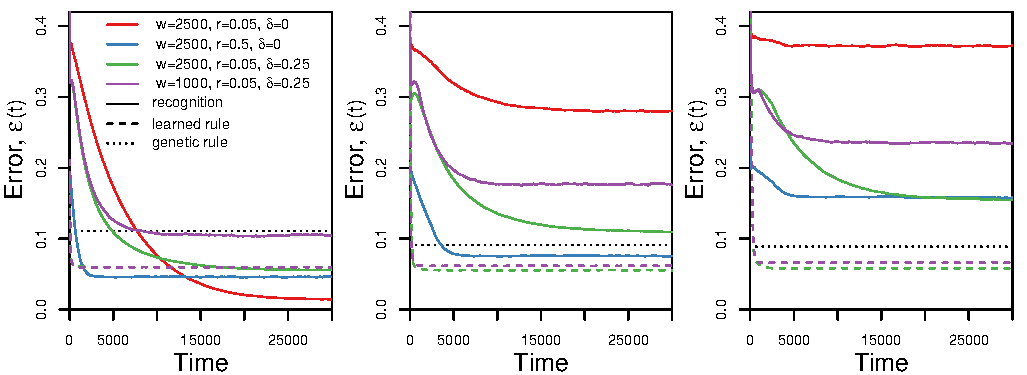
\includegraphics[width=.95\textwidth]{figures/learning_curves.pdf}
\caption{\label{learning_curves} \sffamily\small\textbf{Error decreases over time until it  asymptote.}
In each panel, we show time (in number of interactions) on the x-axis and the average error in an animal's assessments of its peers ($\epsilon(t)$) on the y-axis. In each panel, solid curves show animals using recognition, dashed curves show animals using a learned rule-of-thumb, and dotted curves show animals using a genetic rule-of-thumb. In A, group size $N=25$, in B $N=50$, and in C $N=100$. Each color corresponds to a combination of memory window ($w$), updating rate ($r$), and category width ($\delta$). The signal-quality correlation is high ($\rho=0.99$) in all panels. There are only two dashed curves because $r$ and $\delta$ do not affect a learned rule-of-thumb and there is only one dotted curve because only group size and signal-quality correlation affect a genetic rule-of-thumb. As group size increases (moving from left to right), error increases, but this affects the error of animals using recognition more than animals using either rule-of-thumb. As memory window increases, the error of animals using the learned rule-of-thumb is not strongly affected, but the error of animals using recognition decreases (compare the green and purple curves).}
\end{figure}

\begin{figure}
%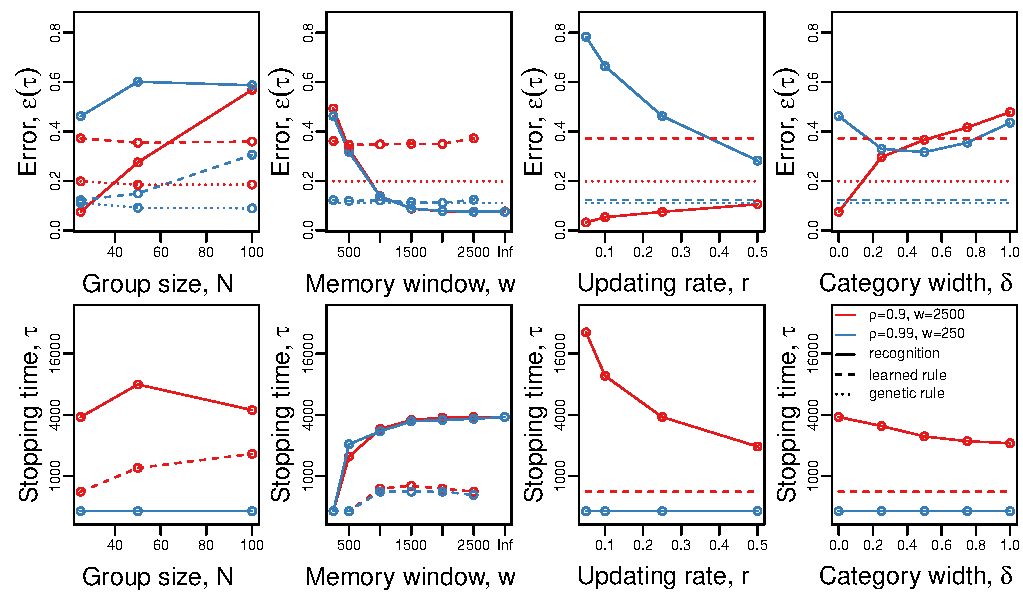
\includegraphics[width=6.85in]{figures/parameters_exploration.pdf}
\caption{\sffamily\small\textbf{Decreasing group size and increasing memory window both improve the accuracy with which animals can learn about their peers.} Here we show average error ($\epsilon(\tau)$) (A-D) and stopping time ($\tau$) (E-H) as a function of group size ($N$), memory window ($w$), updating rate ($r$), and category width ($\delta$). Stopping time is on a logarithmic scale. In each panel, solid curves show animals using recognition, dashed curves show animals using a learned rule-of-thumb, and dotted curves show animals using a genetic rule-of-thumb. The red curves correspond to groups in which the signal-quality correlation $\rho=0.9$ and memory window $w=2500$ and the blue curves correspond to groups in which the signal-quality correlation $\rho=0.99$ and memory window $w=250$. Increasing the updating rate ($r$) helps animals to learn more quickly (C) but increases the error with which they learn when they have long memories (G). Error is minimized at low or intermediate category widths, depending on how long the animals' memory windows are (D). Increasing the category width ($\delta$) helps animals to learn more quickly (H). Parameters: unless the parameter is being varied $\delta = 0$, $N=25$, $r=0.25$.}
\label{parameters}
\end{figure}

\begin{figure}
%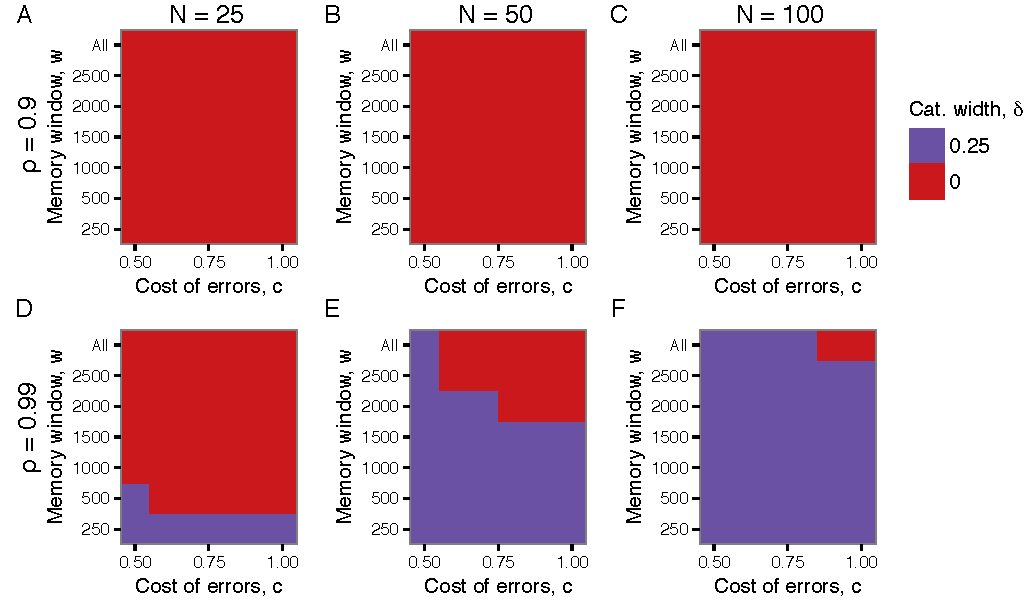
\includegraphics[width=6.85in]{figures/strategies_heat_maps.pdf}
\caption{\sffamily\small\textbf{As the cost of errors increases, animals using recognition should use higher stopping times, smaller updating rates and smaller category widths.} Here we show how the stopping time ($\tau$) (A-C),  optimal updating rate ($r$) (D-F), and optimal category width ($\delta$) (G-I), and error at stopping time ($\epsilon(\tau)$) (J-L), depend on how costly errors are ($c$) and memory window ($w$). Stopping time is on a logarithmic scale. In the first column, group size $N=25$, in the second column $N=50$, and in the third column $N=100$. For a given cost of error ($c$), memory window ($w$), and group size ($N$), the stopping time, updating rate, and category width shown here are those that minimize the costs incurred from the combination error and learning time. Parameters: $\rho=0.99$. }
\label{optimization}
\end{figure}


\begin{figure}
%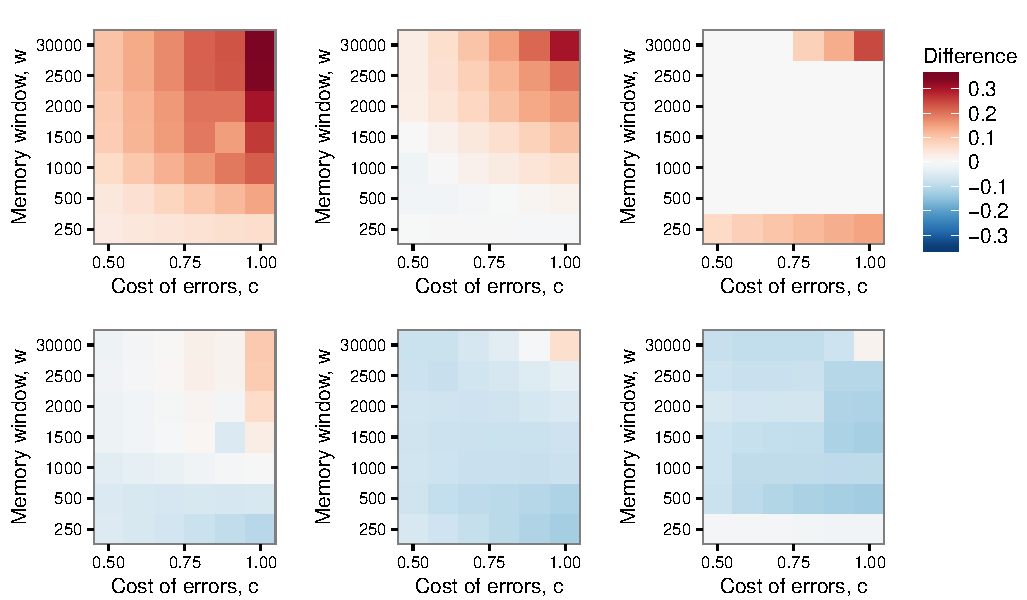
\includegraphics[width=6.85in]{figures/recog_vs_learned_rule.pdf}
\caption{\sffamily\small\textbf{A learned rule-of-thumb is less costly than recognition (with optimized learning strategies) when animals live in large groups and have short memories and when the signal-quality correlation is high.} In each panel, we show the difference in overall costs between recognition and a learned rule-of-thumb as a function of the cost of errors ($c$) and memory window ($w$). Blue indicates a learned rule-of-thumb is less costly and red indicates recognition is less costly. The animals using recognition are using the optimal stopping time ($\tau$), updating rate ($r$), and category width ($\delta$). In the first column $N=25$, in the middle column, $N=50$, and in the right column $N=100$. In the first row $\rho=0.9$ and in the second row $\rho=0.99$.}
\label{comparison}
\end{figure}

\begin{figure}
%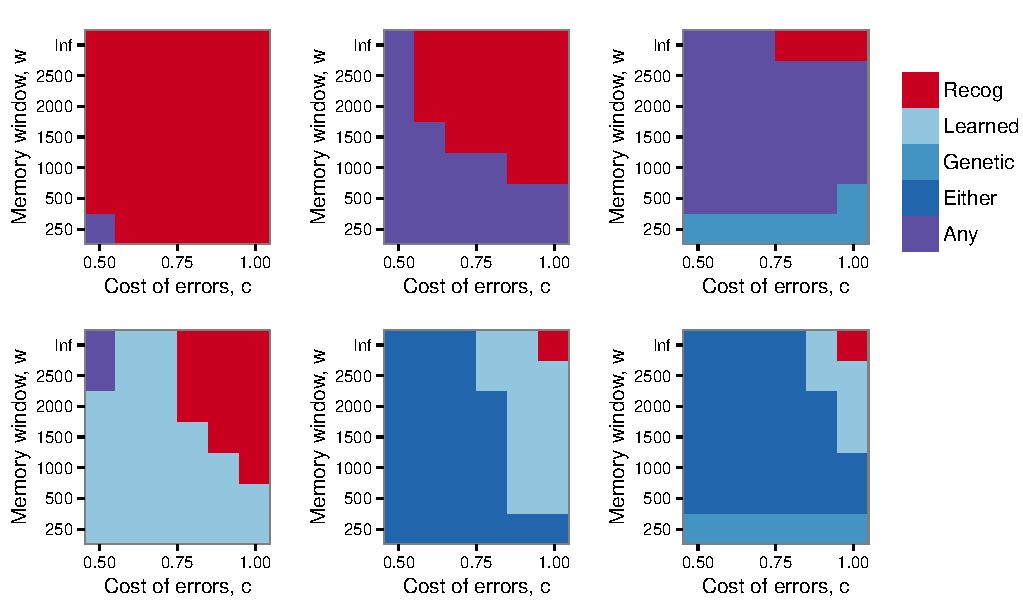
\includegraphics[width=6.85in]{figures/best_type_of_learning.pdf}
\caption{\sffamily\small\textbf{A rule-of-thumb is the best assessment strategy when animals live in large groups and have short memories and when the signal-quality correlation is high.} In each panel, we show which of the three assessment strategies---recognition, a learned rule-of-thumb, or a genetic rule-of-thumb---is the least costly, as a function of the cost of errors ($c$) and memory window ($w$). Red indicates recognition is the least costly. Light blue indicates a learned rule-of-thumb is the best strategy. Intermediate blue indicates a genetic rule-of-thumb is the best strategy. Dark blue indicates the two rule-of-thumbs are essentially equally costly and less costly than recognition. Purple indicates the three strategies are all essentially equally costly. The animals using recognition are using the optimal stopping time ($\tau$), updating rate ($r$), and category width ($\delta$). In the first column $N=25$, in the middle column, $N=50$, and in the right column $N=100$. In the first row $\rho=0.9$ and in the second row $\rho=0.99$.}
\label{best}
\end{figure}

%
\begin {table}[ht]
\caption {Description of variables} \label{tab:vars} 
\begin{tabular}{cl}

 Variables & Description of variables \\
\midrule 
$a_{ij}(t)$ & animal $i$'s assessment of animal $j$ at time $t$ \\
$C(t)$ & total cost of learning \\ 
$c$ & cost of inaccuracy, whereas $1-c$ is the cost of spending time learning \\ 
$\delta$ & category width \\
$e_{ij}(t)$ & error of animal $i$ about animal $j$ at time $t$\\
$\epsilon(t)$ & average error of all animals in all groups at time $t$ \\
$N$ & number of animals in group \\ 
$\mathscr{O}_i(t)$ & set of animals about whom $i$ has an opinion at time $t$\\
$q_i$ & quality of animal $i$ \\ 
$r$ & updating rate\\
$\rho$ & sample correlation between quality and signal in any particular group\\
$s_i$ & signal of quality / badge of status of animal $i$ \\ 
$\sigma_\xi$ & standard deviation of noise in opinion updating during interaction, set to $0.1$ \\
$\sigma_\text{q}$ & standard deviation of quality values, set to $0.5$ \\
$T$ & total number of interactions, set to $30,000$ \\
$\tau$ & stopping time \\
$w$ & memory window \\
$\xi$ & noise in the information animals get about each other's quality through interacting
\end{tabular}
\end {table}
% LIZ comment: add alpha parameter (shape/concavity of cost function?)

\setcounter{figure}{0}
\begin{figure}
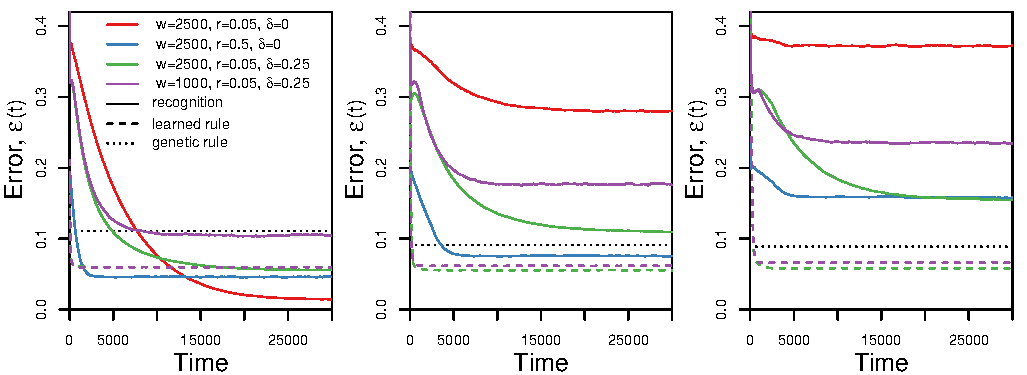
\includegraphics[width=.95\textwidth]{figures/learning_curves.pdf}
\caption{}
\end{figure}


\begin{figure}
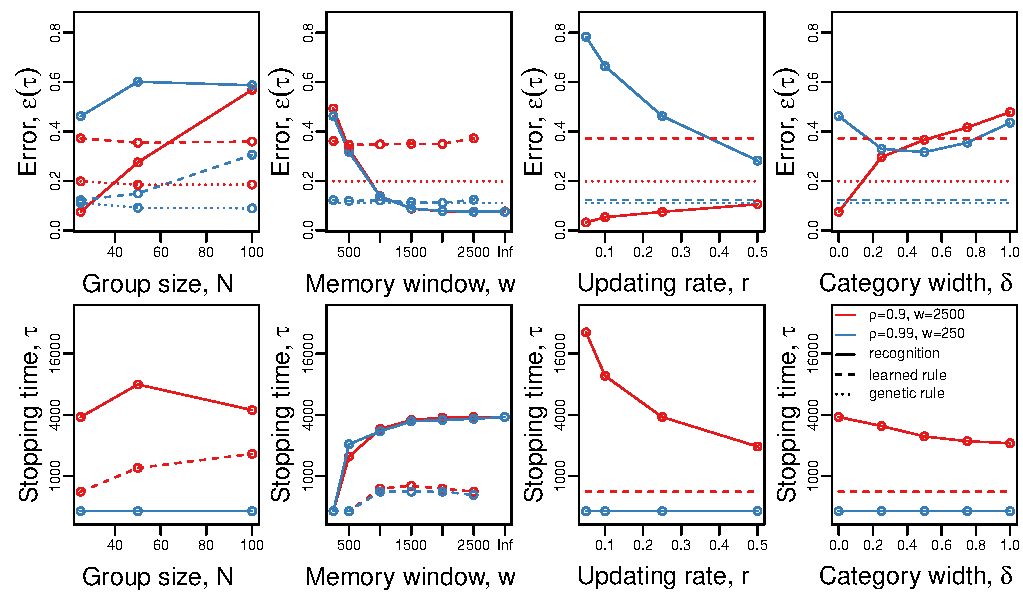
\includegraphics[width=6.85in]{figures/parameters_exploration.pdf}
\caption{}
\end{figure}


\begin{figure}
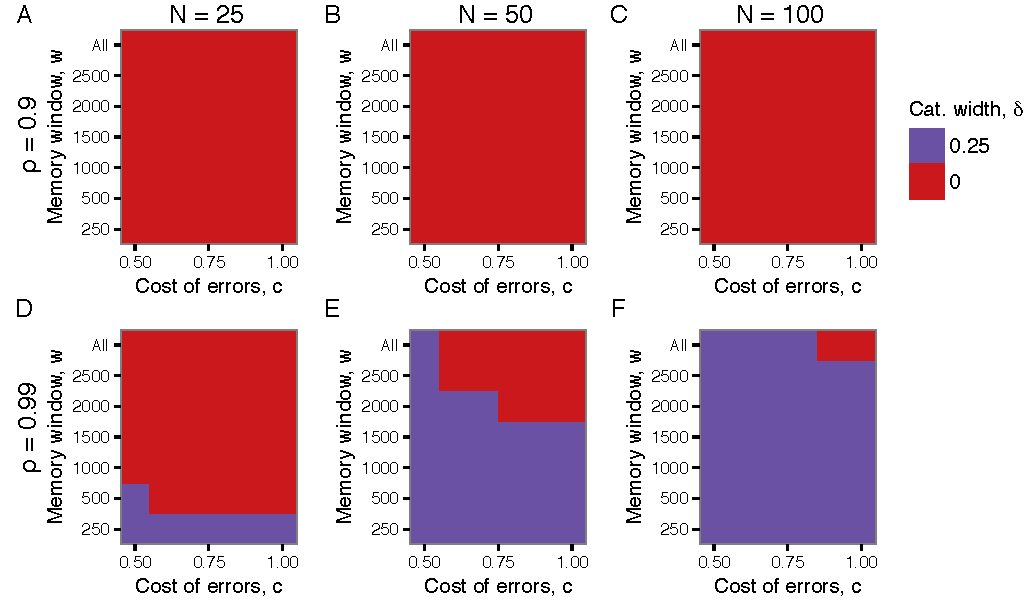
\includegraphics[width=6.85in]{figures/strategies_heat_maps.pdf}
\caption{}
\end{figure}

\begin{figure}
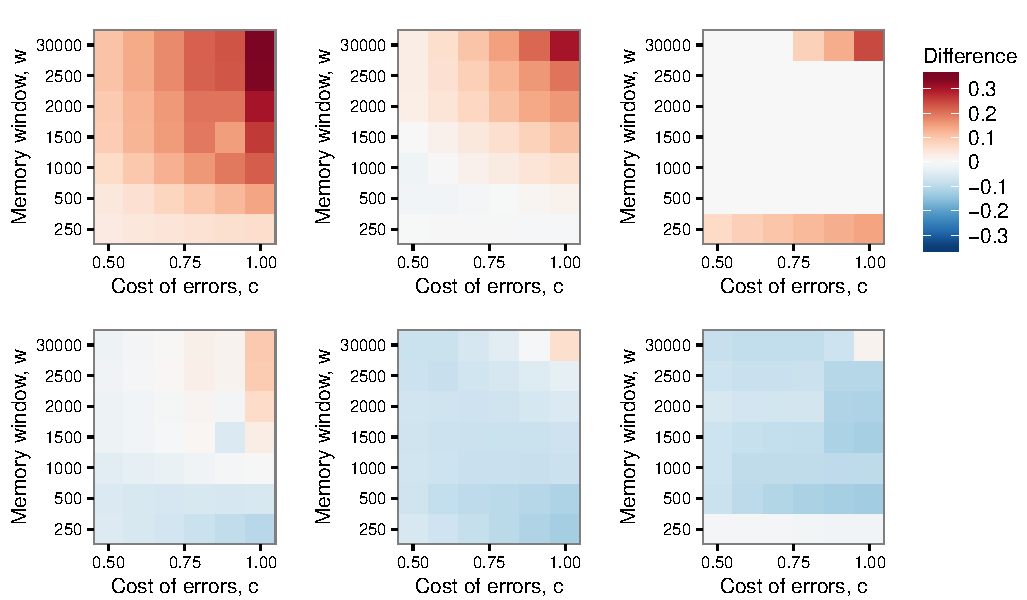
\includegraphics[width=6.85in]{figures/recog_vs_learned_rule.pdf}
\caption{}
\end{figure}

\begin{figure}
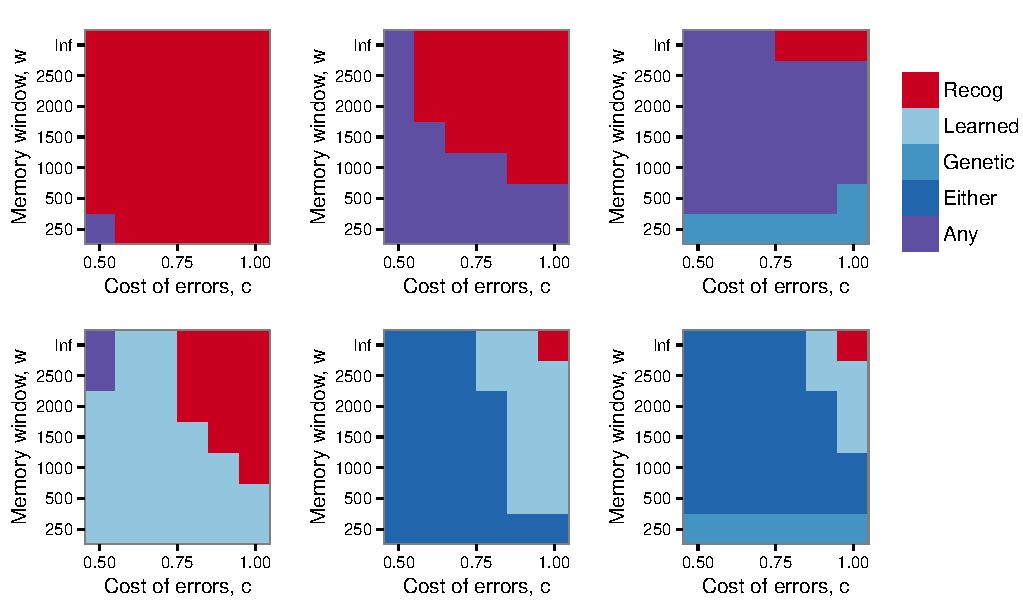
\includegraphics[width=6.85in]{figures/best_type_of_learning.pdf}
\caption{}
\end{figure}

\clearpage{}
%\newpage{}
\renewcommand{\thesection}{}
\section{Supporting information}
\renewcommand{\thesection}{S}
\renewcommand{\thesubsection}{S\arabic{subsection}}
\renewcommand{\theequation}{S\arabic{equation}}
\renewcommand{\thetable}{S\arabic{table}}
\renewcommand{\thefigure}{S\arabic{figure}}
\setcounter{equation}{0}  
\setcounter{figure}{0}
\setcounter{table}{0}

\begin{figure}[ht]
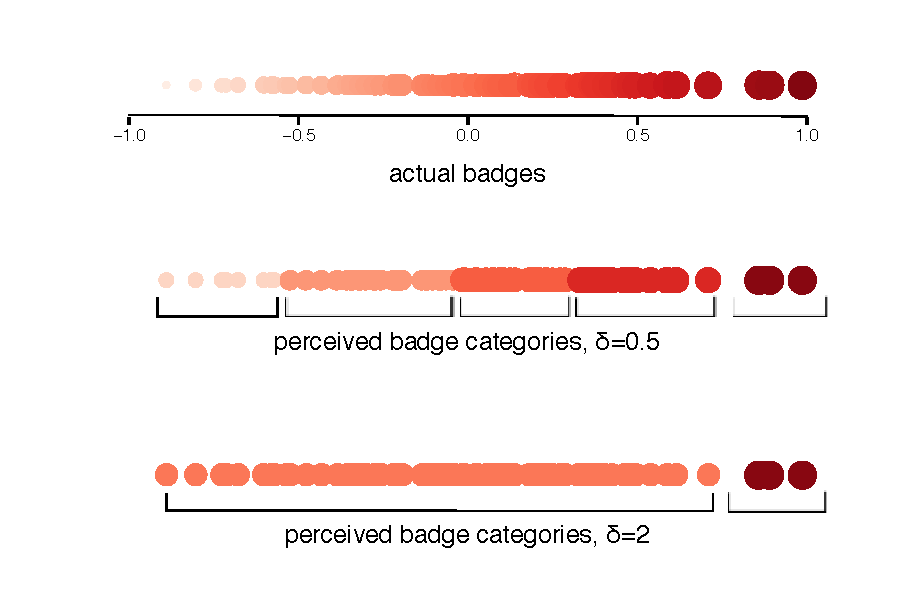
\includegraphics[width=.8\textwidth]{figures/categories.pdf}
\caption{\sffamily\small\textbf{Here we show an example of how a group of $N=100$ animals being divided into categories.} 
Each circle corresponds to an animal in the group. In each row, the horizontal position of the circle corresponds to its badge size. In the top row, the color and size of each circle indicate the size of each animal's badge. In the second and third rows, the color and size indicate the mean size of the badges of animals in each category, where categories were constructed using category width $\delta=0.5$ and $\delta=2$ respectively. Categories were formed by choosing an animal $i$ at random, putting all other animals whose signals were within $\delta/2$ of $i$'s signal $s_i$ into the same category, then choosing another uncategorized animal at random, and continuing until all animals were categorized.}
 \label{cats_ex}
\end{figure}

\begin{figure}[ht]
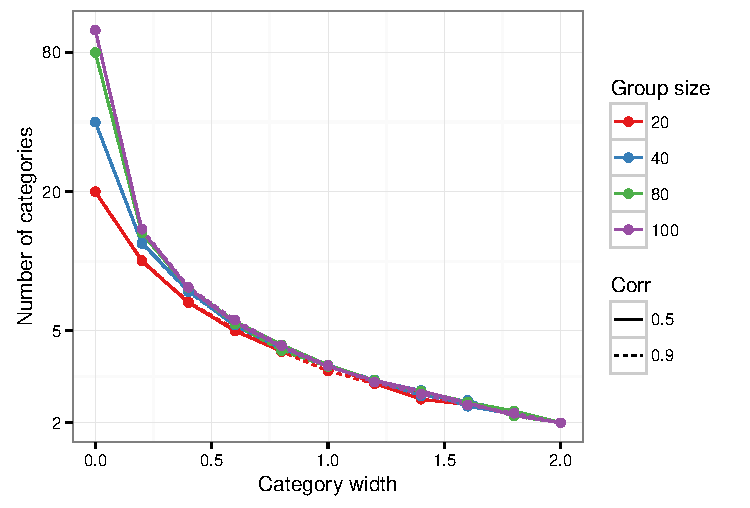
\includegraphics[width=.8\textwidth]{figures/number_of_categories.pdf}
\caption{\sffamily\small\textbf{As category width $\delta$ decreases the number of categories into which the group is divided increases.}
For a given group size ($N$), signal-quality correlation ($\rho$), and category width ($\delta$), we generated $100$ group with signal values $\{s_i\}$ and categorized the group according to the procedure described in the text and shown in Figure \ref{cats_ex}.  Category width is on the x-axis and the average number of categories across the $100$ groups on a logarithmic scale is on the y-axis. Each color corresponds to a group size. Solid curves indicate that $\rho=0.5$ and dashed curves indicate that $\rho=0.9$, but curves overlap since the signal-quality correlation $\rho$ does not affect the number of categories formed. When $\delta=0$ there are as many categories as there are animals in the group. When $\delta=2$, it is theoretically possible for all animals to be put into the same category, but in all $100$ iterations we simulated for each group size, there were $2$ categories. }
\label{num_cat}
\end{figure}

\begin{figure}
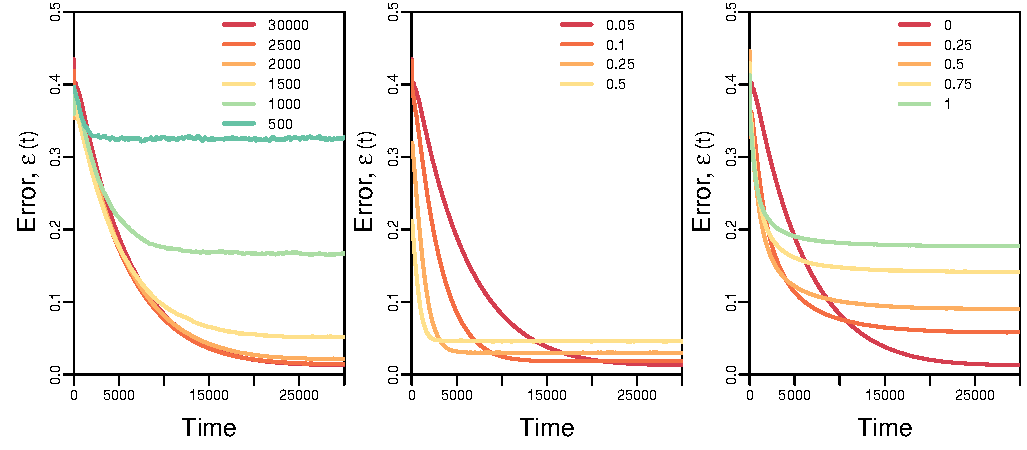
\includegraphics[width=6.85in]{figures/speed_accuracy_tradeoff.pdf}
\caption{\sffamily\small\textbf{Increasing memory always improves learning; increasing updating rate or category width can help animals learn more quickly, but limits how accurately they can learn.} In each panel, we show time (in number of interactions) on the x-axis and the average error in an animal's recognition-based assessment of its peers ($\epsilon(t)$) on the y-axis. In (A), the different curves represent different memory windows ($w$). In (B), the different curves represent different updating rates ($r$). In (C), the different curves represent different category widths ($\delta$). As memory window increases, the learning curves monotonically decrease; there is no benefit to decreasing memory window. As either updating rate or category width increases, the asymptotic error decreases, but error decreases more slowly. If learning quickly is prioritized, it is sometimes desirable to use a large updating rate or category width. Parameters: unless the parameter is being varied $\delta=0$, $N=25$, $\rho=0.99$, $r=0.05$, $w=30000$.}
\label{tradeoff}
\end{figure}


\begin{figure}[ht]
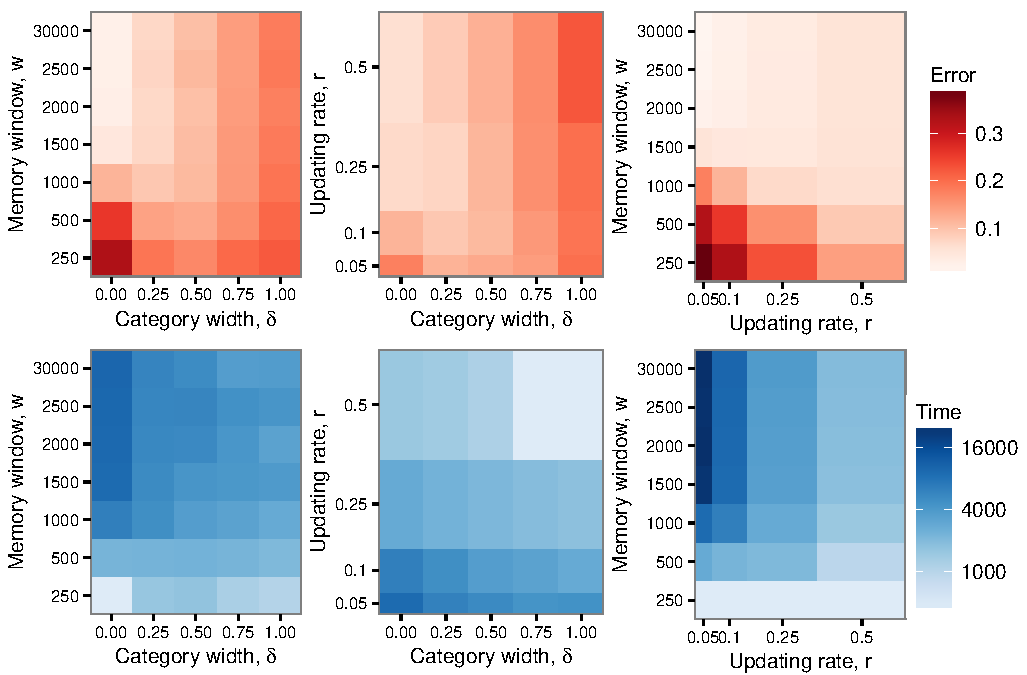
\includegraphics[width=6.85in]{figures/parameters_interactions_full.pdf}
\caption{\sffamily\small\textbf{Memory window, updating rate, and category width interact in their effects on how accurately and quickly animals using recognition can learn.}
In A-C we show average error ($\epsilon(\tau)$) for animals using recognition as a function of two parameters. In D-F we show stopping time ($\tau$) as a function of two parameters. Stopping time is on a logarithmic scale. Increasing memory window always decreases error (A) and increases stopping time (D). Intermediate category widths minimize error when memory and updating rate are low, but otherwise category width $\delta=0$ minimizes error (B). Increasing updating rate always decreases stopping time (F). However, the effects of updating rate depend strongly on memory window: when memory window is low, increasing updating rate decreases error, but when memory window is high, increasing updating rate \emph{increases} error (C). Parameters: unless the parameter is being varied $\delta = 0$, $N=25$, $\rho=0.99$, $w=1000$, $r=0.1$.}
\label{interactions}
\end{figure}

\begin{figure}
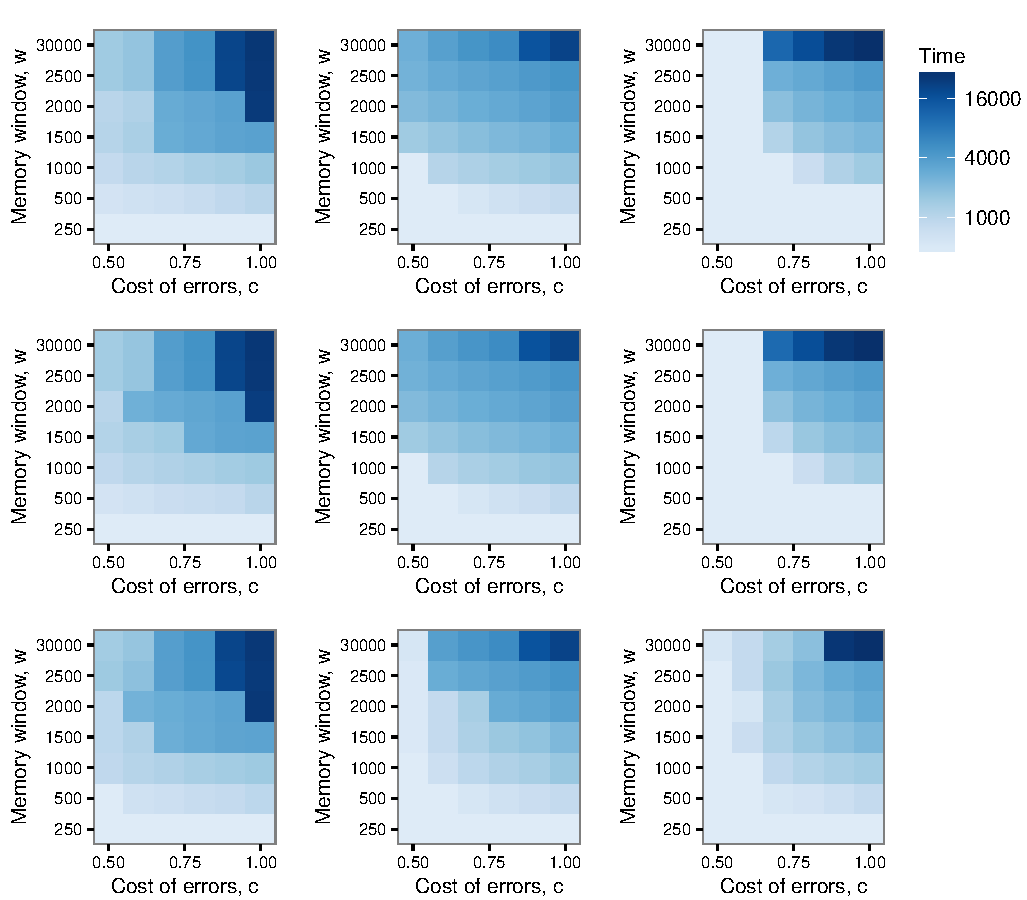
\includegraphics[width=6.85in]{figures/time_heat_maps.pdf}
\caption{\sffamily\small\textbf{} Here we show how the optimal stopping time ($\tau$) depends on the cost of errors ($c$) and memory window ($w$). Stopping time is on a logarithmic scale. In the first column $N=25$, in the middle column $N=50$, and in the right column $N=100$. In the first row $\rho=0.5$, in the second row $\rho=0.9$ and in the third row $\rho=0.99$. The animals are also using the optimal updating rate ($r$) and category width ($\delta$), which are shown in Figures \ref{l} and \ref{delta}.}
\label{time}
\end{figure}

\begin{figure}
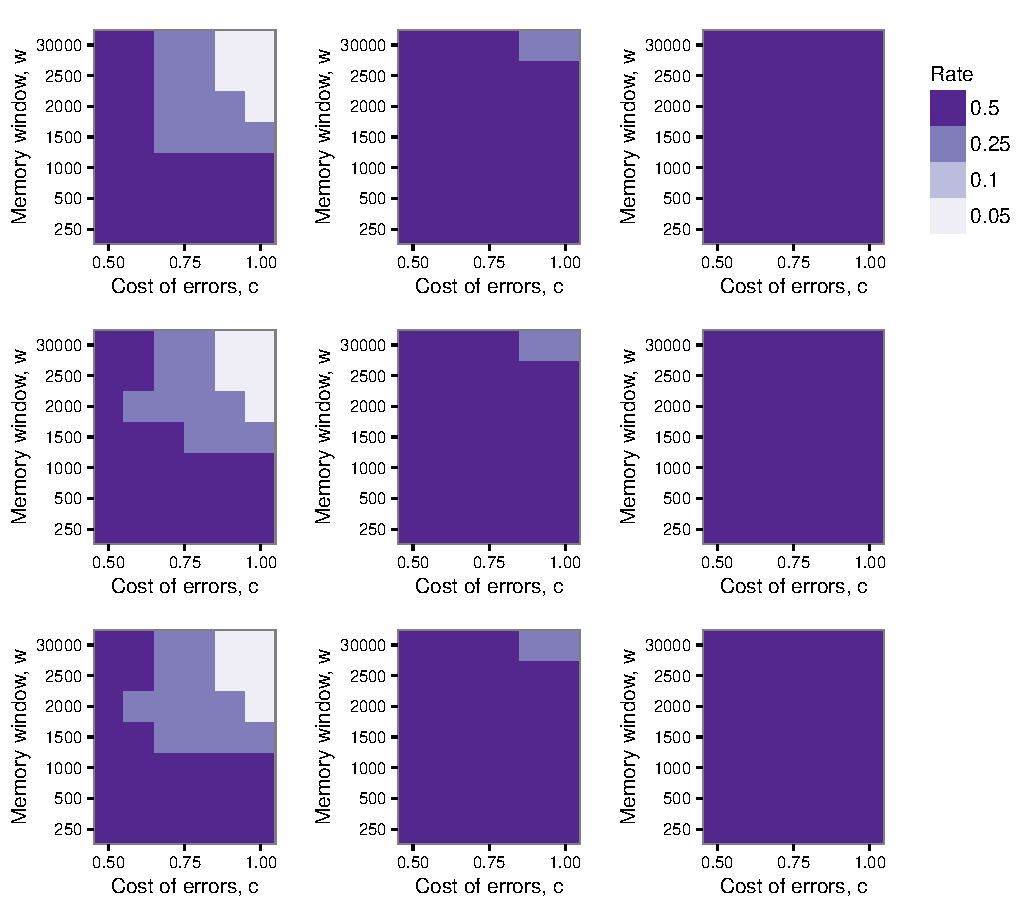
\includegraphics[width=6.85in]{figures/l_heat_maps.pdf}
\caption{\sffamily\small\textbf{A high updating rates is better than a low updating rate when animals live in large groups and have short memory windows.} Here we show how the optimal updating rate ($r$) depends on the cost of errors ($c$) and memory window ($w$). In the first column $N=25$, in the middle column $N=50$, and in the right column $N=100$. In the first row $\rho=0.5$, in the second row $\rho=0.9$, and in the third row $\rho=0.99$. The animals are also using the optimal category width ($\delta$), which is shown in Figure \ref{l}.}
\label{l}
\end{figure} 

\begin{figure}
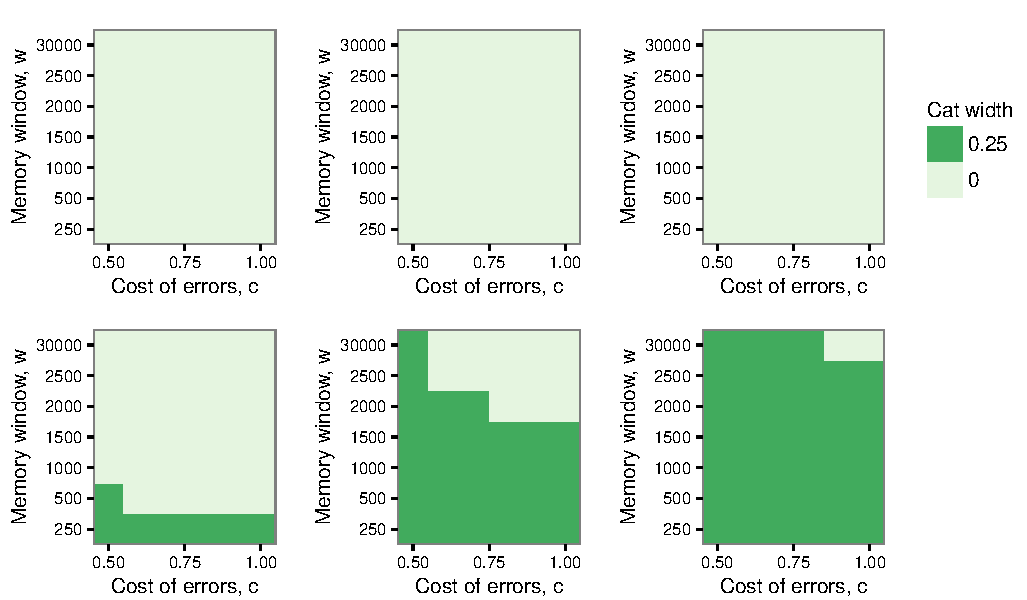
\includegraphics[width=6.85in]{figures/delta_heat_maps.pdf}
\caption{\sffamily\small\textbf{Categorical recognition is better than individual recognition when animals live in large groups and have short memory windows and when the signal-quality correlation is very high.} Here we show how the optimal category width ($\delta$) depends on the cost of errors ($c$) and memory window ($w$). In the first column $N=25$, in the middle column $N=50$, and in the right column $N=100$. In the first row $\rho=0.5$, in the second row $\rho=0.9$, and in the third row $\rho=0.99$. The animals are also using the optimal updating rate ($r$), which is shown in Figure \ref{l}.}
\label{delta}
\end{figure}

\begin{figure}
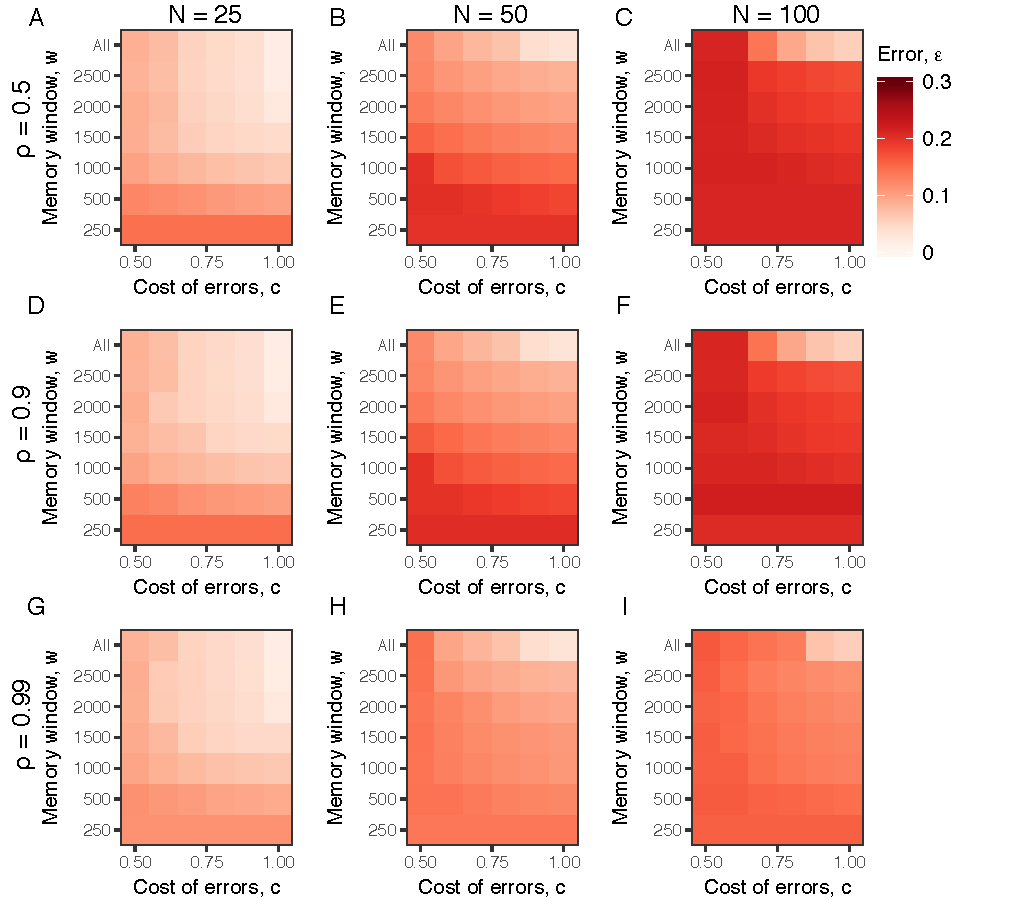
\includegraphics[width=6.85in]{figures/error_heat_maps.pdf}
\caption{\sffamily\small\textbf{} Here we show how the average error ($\epsilon(\tau)$) of animals using optimal stopping time ($\tau$), updating rate ($r$), and category width ($\delta$), depends on the cost of errors ($c$) and memory window ($w$). In the first column $N=25$, in the middle column $N=50$, and in the right column $N=100$. In the first  row $\rho=0.5$, in the second row $\rho=0.9$ and in the third row $\rho=0.99$.}
\label{error}
\end{figure}

\begin{table}
\caption{\label{corr_examples} Examples of the correlation between a badge and a measure of fitness.}
\begin{tabular}{lllll}
Species & Badge & Measure of fitness & Correlation & Reference
\\\hline paper wasp & percent black on face & head width & $r^2=0.36$, for wasps  & Tibbetts \& Dale 2004
\\ & & & with $\geq 2$ black spots
\\ & ``badge brokenness" & dominance & $r^2=.105$ & Tibbetts \& Dale 2004
\\ \hline house sparrow & size of black bib & physical condition & $r=0.379$ & Veiga 1993
\\ \hline swamp sparrow & size of rusty cap & parental investment & $r^2=0.33$ & Olsen et al. 2010
\\ & size of black forehead & aggression & $r^2=0.41$ & Olsen et al. 2010
\end{tabular}
\end{table}

\end{document}
